\documentclass[../main.tex]{subfiles}
\graphicspath{{\subfix{../images/}}}
\begin{document}

Various elements of an orbit can now be expressed simply. Note that there is a lot of variation in standards when it comes to hyperbolas and parabolas. In this document, the convention will be used that $a, c<0$ in a hyperbola. Note that $p$ is always positive. In a parabola, $a$ is infinite.

Throughout this section, it will be shown that an orbit can be defined uniquely by $a$ and $e$ (except for parabolic orbits).

\bigskip\bigskip
\subsection{Periapsis}\label{sec:Periapsis Geometric}

From Figure \ref{fig:Orbit Diagram}, a geometric observation can be made.
\begin{align*}
    r_\text{pe}+c+a & = 2a     \\
    r_\text{pe}     & =a-c     \\
                    & =a-ea    \\
                    & = a(1-e)
\end{align*}

TThis equation is valid for all elliptic and hyperbolic orbits, but not for parabolic ones (the semi-major axis of a parabola is infinite, while $1-e$ equals zero in a parabola).
\begin{equation}\label{Periapsis Radius Geometric}
    r_\text{pe}=a(1-e)
\end{equation}

\bigskip\bigskip
\subsection{Apoapsis}\label{sec:Apoapsis Geometric}

Using the same figure and similar observations and reasoning, the apoapsis radius can be found.
\begin{align*}
    r_\text{ap} & = a+c   \\
                & =a+ea   \\
                & =a(1+e)
\end{align*}

The apoapsis is not defined for hyperbolic or parabolic orbits.
\begin{equation}\label{Apoapsis Radius Geometric}
    r_\text{ap}=a(1+e)
\end{equation}

\bigskip\bigskip
\subsection{Semi-Minor Axis}\label{Sec:Semi Minor Axis Geometric}

The Semi-Minor Axis $b$ is slightly harder to find than the apoapsis and periapsis. Of course, various definitions of eccentricity can be applied, such as $e=\sqrt{1-\frac{a^2}{b^2}}$, to solve for $b$, however that's not quite intellectually fulfilling; after all, it's not immediately obvious where that equation came from.

Instead, the definition of an ellipse wil be brought in. In a circle, the distance to the center is always constant. In an ellipse, the sum of distances to the foci is always constant. This distance will be denoted $2d$.
\begin{align*}
    2d(\text{At Pe}) & = r_\text{pe}+(r_\text{ap}) \\
                     & = 2a                        \\
    d                & =a
\end{align*}

A right triangle can then be drawn with which further reasoning can be applied
\begin{figure}[H]
    \centering
    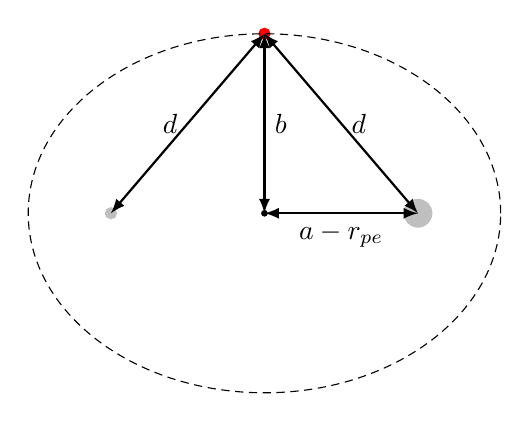
\begin{tikzpicture}[>=latex]
        \def\ecc{0.65}
        \def\SMA{3}
        \def\ap{\fpeval{\SMA*(1+\ecc)}}
        \def\pe{\fpeval{\SMA*(1-\ecc)}}
        \def\slr{\fpeval{\SMA*(1-(\ecc)^2)}}
        \def\SmA{\fpeval{\SMA*sqrt(1-\ecc^2)}}

        \filldraw[lightgray] (-\ap+\SMA,0) circle (2pt);
        \filldraw[lightgray] (-\SMA+\ap,0) circle (5pt);
        \filldraw[] (0,0) circle (1pt);
        \filldraw[red] (0,\SmA) circle (2pt);

        \draw[thin, densely dashed] (0,0) ellipse ({\SMA} and {\SmA});
        \draw[<->, thick] (0, 0) -- (\SMA-\pe, 0) node[midway, below] {$a-r_\text{pe}$};
        \draw[<->, thick] (0, 0) -- (0, \SmA) node[midway, right] {$b$};

        \draw[<->, thick] (-\ap+\SMA, 0) -- (0, \SmA) node[midway, left] {$d$};
        \draw[<->, thick] (\ap-\SMA, 0) -- (0, \SmA) node[midway, right] {$d$};

    \end{tikzpicture}

    \caption{An orbit with relevant parameters labeled, and with the point on the semi-major axis drawn in red}. The vacant focus is the smaller circle, with the orbited body being the large gray circle.
\end{figure}

The right triangle that will be examined is the one formed by the center of the orbit, the left focus, and the point in the orbit on the semi-minor axis. The Pythagorean Theorem can be applied to find the unknown $b$, keeping in mind that $d=a$.
\begin{align*}
    (a-r_\text{pe})^2+b^2 & = d^2                   \\
    (a-r_\text{pe})^2+b^2 & = a^2                   \\
    b^2                   & = a^2-(a-r_\text{pe})^2 \\
\end{align*}

Note from Figure \ref{fig:Orbit Diagram} that $r_\text{pe}+c=a$, meaning that $a-r_\text{pe}=c$, which in turn is defined as $c=ae$
\begin{align*}
    b^2 & = a^2-(c)^2         \\
    b^2 & = a^2-(ae)^2        \\
    b^2 & = a^2-a^2e^2        \\
    b^2 & = a^2(1-e^2)        \\
    b   & = \sqrt{a^2(1-e^2)} \\
    b   & = a\sqrt{1-e^2}     \\
\end{align*}

The semi-minor axis is not well defined for hyperbolic orbits. The argument of the square root can be put in an absolute value to ensure that the semi-minor axis is real. Note that for some hyperbolic orbits (namely where $e>\sqrt{2}$), $|b|>|a|$.

\begin{equation}\label{Semi Minor Axis Geometric}
    b=a\sqrt{|1-e^2|}
\end{equation}

\bigskip\bigskip
\subsection{Geometry in Terms of Measurable Parameters}\label{sec:Geometry in terms of Measurable Values}

While $e$ and $a$ are conventionally used as the defining parameters of an orbit, the apses can instead be used to describe elliptic orbits. Once $e$ and $a$ are known, other geometric parameters can be found as before. Hyperbolic and parabolic orbits do not have a defined apoapsis, so this does not apply to them.

\subsubsection{Semi-Major Axis in terms of Apses}
From Figure \ref{fig:Orbit Diagram}, $a$ can be found in terms of $r_\text{pe}$ and $r_\text{ap}$

\begin{align*}
    2a & = r_\text{pe}+r_\text{ap}
\end{align*}
\begin{equation}\label{SMA in terms of apses}
    a = \frac{r_\text{pe}+r_\text{ap}}{2}
\end{equation}

\subsubsection{Eccentricity in Terms of Apses}

The eccentricity can also be put in terms of $r_\text{ap}$ and $r_\text{pe}$ using Equations \eqref{Periapsis Radius Geometric} and \eqref{Apoapsis Radius Geometric}.
\begin{align*}
    r_\text{ap}             & =a(1+e) & r_\text{pe}             & =a(1-e) \\
    \frac{r_\text{ap}}{1+e} & =a      & \frac{r_\text{pe}}{1-e} & =a      \\
\end{align*}

Setting both sides equal to eachother,

\begin{align*}
    \frac{r_\text{ap}}{1+e}                                   & =\frac{r_\text{pe}}{1-e}                                                                                                                                                             \\
    \frac{1+e}{r_\text{ap}}                                   & =\frac{1-e}{r_\text{pe}}                                                                                                                                                             \\
    \frac{1}{r_\text{ap}}+\frac{e}{r_\text{ap}}               & =\frac{1}{r_\text{pe}}-\frac{e}{r_\text{pe}}                                                                                                                                         \\
    \frac{e}{r_\text{ap}}+\frac{e}{r_\text{pe}}               & =\frac{1}{r_\text{pe}}-\frac{1}{r_\text{ap}}                                                                                                                                         \\
    e\left(\frac{1}{r_\text{ap}}+\frac{1}{r_\text{pe}}\right) & =\frac{1}{r_\text{pe}}-\frac{1}{r_\text{ap}}                                                                                                                                         \\
    e                                                         & =\frac{\frac{1}{r_\text{pe}}-\frac{1}{r_\text{ap}}}{\frac{1}{r_\text{pe}}+\frac{1}{r_\text{ap}}}                                                                                     \\
                                                              & =\frac{\frac{r_\text{pe}r_\text{ap}}{r_\text{pe}}-\frac{r_\text{pe}r_\text{ap}}{r_\text{ap}}}{\frac{r_\text{pe}r_\text{ap}}{r_\text{pe}}+\frac{r_\text{pe}r_\text{ap}}{r_\text{ap}}} \\
                                                              & =\frac{r_\text{ap}-r_\text{pe}}{r_\text{ap}+r_\text{pe}}                                                                                                                             \\
\end{align*}
\begin{equation}\label{Accentricity in terms of apses}
    e=\frac{r_\text{ap}-r_\text{pe}}{r_\text{ap}+r_\text{pe}}
\end{equation}

\bigskip\bigskip
\subsection{Conclusion}

Throughout this section, many geometric relationships have been found describing orbits. Most importantly, it has been shown that an orbital trajectory can be described in its plane using only two parameters: the semi-major axis $a$ and the eccentricity $e$. These relationships are summarized here.

\bigskip
The periapsis and apoapsis radii are
$$r_\text{pe}=a(1-e)\qquad\text{and}\qquad r_\text{ap}=a(1+e)$$

\bigskip
The semi-minor axis of the orbit is
$$b=a\sqrt{|1-e^2|}$$

\bigskip
The semi-major axis and eccentricity of an elliptic orbit can be stated in terms of known periapsis and apoapsis radii
$$a=\frac{r_\text{pe}+r_\text{ap}}{2}\qquad\qquad e=\frac{r_\text{ap}-r_\text{pe}}{r_\text{ap}+r_\text{pe}}$$

Because hyperbolas don't have physically meaningful apoapses, the semi-major axis and eccentricity can be defined in terms of the entry/exit angle $\theta_\text{hyp}$ and the periapsis radius.
$$e=\sec(\theta_\text{hyp})\qquad\qquad a=\frac{{r_\text{pe}}}{1-\sec(\theta_\text{hyp})}$$
\end{document}